
\subsection{Especificación del modelo de clases}
\label{especificacion-modelo-clases}
\subsubsection{Análisis de clases}

El siguiente paso después de la creación de los casos de usos consiste en pensar qué elementos van a intervenir en el sistema, para que el comportamiento y servicios que se describen en la sección \emph{Análisis del sistema} \ref{analisis-del-sistema} puedan realizarse.

Estos elementos en UML son las clases y son el primer nivel (nivel más bajo y con grano más fino) de todos los elementos que intervienen en el análisis de la aplicación.

Dada la naturaleza del sistema, subyacen dos diagramas de clase separados, con las respectivas clases que los componen:
\begin{itemize}
    \item Diagrama del sistema general.
    \begin{itemize}
        \item Sistema.
        \item Ayuda.
        \item EvaluadorPiezaGenerada.
        \item SelectorGéneroMusical.
        \item ModeloGeneradorMúsica.
        \item PiezaMusical.
    \end{itemize}
    \item Diagrama del modelo de Inteligencia Artificial.
    \begin{itemize}
        \item CargadorMP3.
        \item PiezaMusicalEtiquetada.
        \item ModeloGeneradorIA.
        \item VAE.
        \item GAN.
        \item Transformer.
    \end{itemize}
\end{itemize}

\begin{enumerate}

  \item \textbf{Clase Sistema}

  La clase ``Sistema'' representa el conjunto general del sistema, es decir, la clase principal de la aplicación.

  Los métodos de la clase son:

  \begin{itemize}
      \item init: inicia la aplicación informática.
  \end{itemize}

  \begin{figure}[H]
    \centering
    \includesvg[width=0.2\textwidth]{images/clase-sistema.svg}
    \caption{Clase Sistema.}
  \end{figure}


  \item \textbf{Clase Ayuda}

  La clase ``Ayuda'' representa a la ayuda sobre el uso de la aplicación.

  Esta clase cuenta con el siguiente método:

  \begin{itemize}
      \item motrarAyuda: muestra la ayuda de la aplicación.
  \end{itemize}

  \begin{figure}[H]
    \centering
    \includesvg[width=0.3\textwidth]{images/clase-ayuda.svg}
    \caption{Clase Ayuda.}
  \end{figure}

  \item \textbf{Clase SelectorGeneroMusical}

  La clase ``SelectorGeneroMusical'' representa el selector de géneros musicales disponibles.

  Esta clase tiene el siguiente método:

  \begin{itemize}
      \item devolverGeneroMusicalSeleccionado: devuelve el género musical que el usuario ha seleccionado.
  \end{itemize}

  \begin{figure}[H]
    \centering
    \includesvg[width=0.5\textwidth]{images/clase-selector-genero-musical.svg}
    \caption{Clase SelectorGeneroMusicalSeleccionado.}
  \end{figure}


  \item \textbf{Clase EvaluadorPiezaGenerada}

  La clase ``EvaluadorPiezaGenerada'' representa el lugar donde el usuario emitirá una evaluación sobre la pertenencia de la pieza generada, al género demandado.

  Esta clase cuenta con el siguiente método:

  \begin{itemize}
      \item asignarEvaluacion: recoge la evaluación emitida por el usuario.
  \end{itemize}

  \begin{figure}[H]
    \centering
    \includesvg[width=0.5\textwidth]{images/clase-evaluador-pieza-generada.svg}
    \caption{Clase EvaluadorPiezaGenerada.}
  \end{figure}

  \item \textbf{Clase PiezaMusical}

  La clase ``PiezaMusical'' representa una pieza musical. Esta clase será la abstracción de un fichero MP3 en el sistema.

  \begin{figure}[H]
    \centering
    \includesvg[width=0.2\textwidth]{images/clase-pieza-musical.svg}
    \caption{Clase PiezaMusical.}
  \end{figure}

  \item \textbf{Clase ModeloGeneradorMusical}

  La clase ``ModeloGeneradorMusical'' representa el modelo de Inteligencia Artificial capaz de generar piezas de música bajo demanda, con un género concreto.

  La clase ``ModeloGeneradorMusical'' cuenta con el siguiente método:

  \begin{itemize}
      \item devolverPiezaMusical: devuelve una pieza musical del género demandado.
  \end{itemize}

  \begin{figure}[H]
    \centering
    \includesvg[width=0.5\textwidth]{images/clase-modelo-generador-musical.svg}
    \caption{Clase ModeloGeneradorMusical.}
  \end{figure}

  A continuación, se exponen las clases que aparecen dentro e integran el modelo de Inteligencia Artificial descrito en esta última clase nombrada ``ModeloGeneradorMusical''.

  \item \textbf{Clase PiezaMusicalEtiquetada}

  La clase ``PiezaMusicalEtiquetada'' representa una pieza musical, junto a su etiqueta de género asociada. Esta clase será la abstracción de un fichero MP3 en el sistema, utilizado para entrenar el modelo de Inteligencia Artificial. Esta clase hereda todos los comportamientos de su clase padre ``PiezaMusical''.

  La clase ``PiezaMusicalEtiquetada'' cuenta con el siguiente atributo:

  \begin{itemize}
      \item genero: etiqueta de género.
  \end{itemize}

  La clase tiene el siguiente método:

  \begin{itemize}
      \item devolverGenero: devuelve el valor de la etiqueta de género.
  \end{itemize}

  \begin{figure}[H]
    \centering
    \includesvg[width=0.4\textwidth]{images/clase-pieza-musical-etiquetada.svg}
    \caption{Clase PiezaMusicalEtiquetada.}
  \end{figure}

  \item \textbf{Clase CargadorMP3}

  La clase ``CargadorMP3'' representa un \textbf{generador} bajo demanda de la representación numérica de una pieza musical, con una etiqueta de género asociada.
  La clase ``CargadorMP3'' cuenta con el siguiente método:

  \begin{itemize}
      \item generarPiezaMusical: devuelve una pieza musical etiquetada, generada bajo demanda.
  \end{itemize}

  \begin{figure}[H]
    \centering
    \includesvg[width=0.5\textwidth]{images/clase-cargador-mp3.svg}
    \caption{Clase CargadorMP3.}
  \end{figure}

  \item \textbf{Clase ModeloGeneradorIA}

  La clase ``ModeloGeneradorIA'' conforma la clase padre que abstrae el comportamiento del modelo de Inteligencia Artificial dentro del sistema.

  La clase tiene los siguientes métodos:

  \begin{itemize}
      \item devolverPiezaMusical: devuelve una pieza musical del género demandado.
      \item devolverError: devuelve el error cometido entre la pieza generada y la pieza musical a comparar.
  \end{itemize}

  \begin{figure}[H]
    \centering
    \includesvg[width=0.4\textwidth]{images/clase-modelo-generador-ia.svg}
    \caption{Clase ModeloGeneradorIA.}
  \end{figure}


  \item \textbf{Clase VAE}

  La clase ``VAE'' representa el modelo de \emph{Variational AutoEncocder} de Inteligencia Artificial.

  Esta clase servirá para establecer una comparativa entre lo generado por el modelo \emph{GAN} y por el modelo \emph{VAE}.

  Hereda todos los comportamientos de la clase padre ``ModeloGeneradorIA''.

  \begin{figure}[H]
    \centering
    \includesvg[width=0.07\textwidth]{images/clase-vae.svg}
    \caption{Clase VAE.}
  \end{figure}

  \item \textbf{Clase GAN}

  La clase ``GAN'' representa el modelo de \emph{Generative Adversarial Network} de Inteligencia Artificial.

  Esta clase servirá para generar muestras musicales bajo demanda, de un género musical concreto.

  Hereda todos los comportamientos de la clase padre ``ModeloGeneradorIA''.

  \begin{figure}[H]
    \centering
    \includesvg[width=0.07\textwidth]{images/clase-gan.svg}
    \caption{Clase GAN.}
  \end{figure}

  \subsubsection{Análisis de relaciones}

  En esta sección se describen las relaciones que cada clase tiene con las demás. El análisis se efectuará en primera instancia orientado a cada relación y después se mostrará un diagrama de relaciones completo de todas las clases.

  \item \textbf{Sistema - Ayuda}

  Representa la relación unidireccional entre la clase Ayuda y la
  clase Sistema, en la cual la clase Sistema consulta a la clase
  Ayuda.

  \begin{figure}[H]
    \centering
    \includesvg[width=0.4\textwidth]{images/relacion-ayuda-sistema.svg}
    \caption{Relación Sistema - Ayuda.}
  \end{figure}

  \item \textbf{SelectorGeneroMusical - Sistema}

  Representa la relación unidireccional existente entre las clases SelectorGeneroMusical y Sistema, en la que el sistema solicita el género de música de la pieza que se quiere generar.

  \begin{figure}[H]
    \centering
    \includesvg[width=0.6\textwidth]{images/relacion-selector-genero-musical-sistema.svg}
    \caption{Relación SelectorGeneroMusical - Sistema.}
  \end{figure}

  \item \textbf{EvaluadorPiezaGenerada - Sistema}

  Representa la relación unidireccional existente entre las clases EvaluadorPiezaGenerada y Sistema, que permitirá emitir una valoración de pertenencia de la pieza musical generada con respecto al género solicitado.

  \begin{figure}[H]
    \centering
    \includesvg[width=0.6\textwidth]{images/relacion-sistema-evaluador-pieza-musical.svg}
    \caption{Relación EvaluadorPiezaGenerada - Sistema.}
  \end{figure}

  \item \textbf{ModeloGeneradorMúsica - Sistema}

  Representa la relación unidireccional existente entre las clases ModeloGeneradorMúsica y Sistema, que permitirá al sistema generar música bajo demanda.

  \begin{figure}[H]
    \centering
    \includesvg[width=0.6\textwidth]{images/relacion-sistema-modelo-generador-musica.svg}
    \caption{Relación ModeloGeneradorMúsica - Sistema.}
  \end{figure}

  \item \textbf{PiezaMusical - ModeloGeneradorMúsica}

  Representa la relación unidireccional existente entre las clases PiezaMusical y ModeloGeneradorMúsica. Esta relación representa la generación de varias piezas musicales por parte del Sistema.

  \begin{figure}[H]
    \centering
    \includesvg[width=0.6\textwidth]{images/relacion-modelo-generador-musica-pieza-musical.svg}
    \caption{Relación PiezaMusical- ModeloGeneradorMúsica.}
  \end{figure}

  Las siguiente relaciones se dan dentro de la abstracción contenida en la clase ModeloGeneradorMúsica, la cual explica la arquitectura interna del modelo de Inteligencia Artificial.

  \item \textbf{VAE - ModeloGeneradorIA}

  De manera análoga a la relación anterior, ésta representa la relación de herencia entre las clases VAE y ModeloGeneradorIA. La clase VAE hereda todos los comportamientos de la clase ModeloGeneradorIA.

  \begin{figure}[H]
    \centering
    \includesvg[width=0.6\textwidth]{images/relacion-modelo-generador-ia-vae.svg}
    \caption{Relación VAE - ModeloGeneradorIA.}
  \end{figure}

  \item \textbf{GAN - ModeloGeneradorIA}

  Representa la relación de herencia entre las clases GAN y ModeloGeneradorIA. La clase GAN hereda todos los comportamientos de la clase ModeloGeneradorIA.

  \begin{figure}[H]
    \centering
    \includesvg[width=0.6\textwidth]{images/relacion-modelo-generador-ia-gan.svg}
    \caption{Relación GAN - ModeloGeneradorIA.}
  \end{figure}

  \item \textbf{Transformer - GAN}

  El elemento Transformer pertenece a un único elemento GAN. Un modelo GAN contiene uno y sólo un elemento Transformer, que será su elemento generador.

  \begin{figure}[H]
    \centering
    \includesvg[width=0.6\textwidth]{images/relacion-gan-transformer.svg}
    \caption{Relación Transformer - GAN.}
  \end{figure}

  \item \textbf{PiezaMusicalEtiquetada - PiezaMusical}

  Representa la relación de herencia entre las clases PiezaMusicalEtiquetada y PiezaMusical. La clase PiezaMusicalEtiquetada hereda todos los comportamientos de la clase PiezaMusical.

  \begin{figure}[H]
    \centering
    \includesvg[width=0.3\textwidth]{images/relacion-pieza-musical-etiquetada-pieza-musical.svg}
    \caption{Relación PiezaMusicalEtiquetada - PiezaMusical.}
  \end{figure}

  \item \textbf{PiezaMusicalEtiquetada - CargadorMP3}

  Todo elemento PiezaMusicalEtiquetada pertenece a un único elemento CargadorMP3. El elemento cargador de piezas musicales de entrenamiento MP3 contiene una o más representaciones de dichas piezas, que están en un único elemento cargador.

  \begin{figure}[H]
    \centering
    \includesvg[width=0.58\textwidth]{images/relacion-cargadormp3-pieza-musical-etiquetada.svg}
    \caption{Relación PiezaMusicalEtiquetada - CargadorMP3.}
  \end{figure}

  \item \textbf{VAE - CargadorMP3}

  Representa la relación unidireccional existente entre las clases VAE y CargadorMP3, que permitirá al modelo generador accede a información para el entrenamiento.

  \begin{figure}[H]
    \centering
    \includesvg[width=0.35\textwidth]{images/relacion-vae-cargadormp3.svg}
    \caption{Relación VAE - CargadorMP3.}
  \end{figure}

  \item \textbf{GAN - CargadorMP3}

  Representa la relación unidireccional existente entre las clases GAN y CargadorMP3, que permitirá al modelo generador accede a información para el entrenamiento.

  \begin{figure}[H]
    \centering
    \includesvg[width=0.35\textwidth]{images/relacion-gan-cargadormp3.svg}
    \caption{Relación GAN - CargadorMP3.}
  \end{figure}

  \subsubsection{Diagrama de clases del sistema}

  Como ya se ha mencinado anteriormente, dada la naturaleza del sistema, subyacen dos diagramas de clase separados.

  Uno de ellos muestra el diagrama general del sistema y el otro muestra la relación de clases que conciernen al entrenamiento del modelo de Inteligencia Artificial. Además de ello, existe un tercer diagrama de clases que integra a los dos y resuelve la abstracción del modelo entrenado del primer diagrama.

  \item \textbf{Diagrama de clases general del sistema}

  \begin{figure}[H]
    \centering
    \includesvg[width=0.93\textwidth]{images/diagrama-clases-general.svg}
    \caption{Diagrama de clases general del sistema.}
  \end{figure}

  \item \textbf{Diagrama de clases del modelo de Inteligencia Artificial}

  \begin{figure}[H]
    \centering
    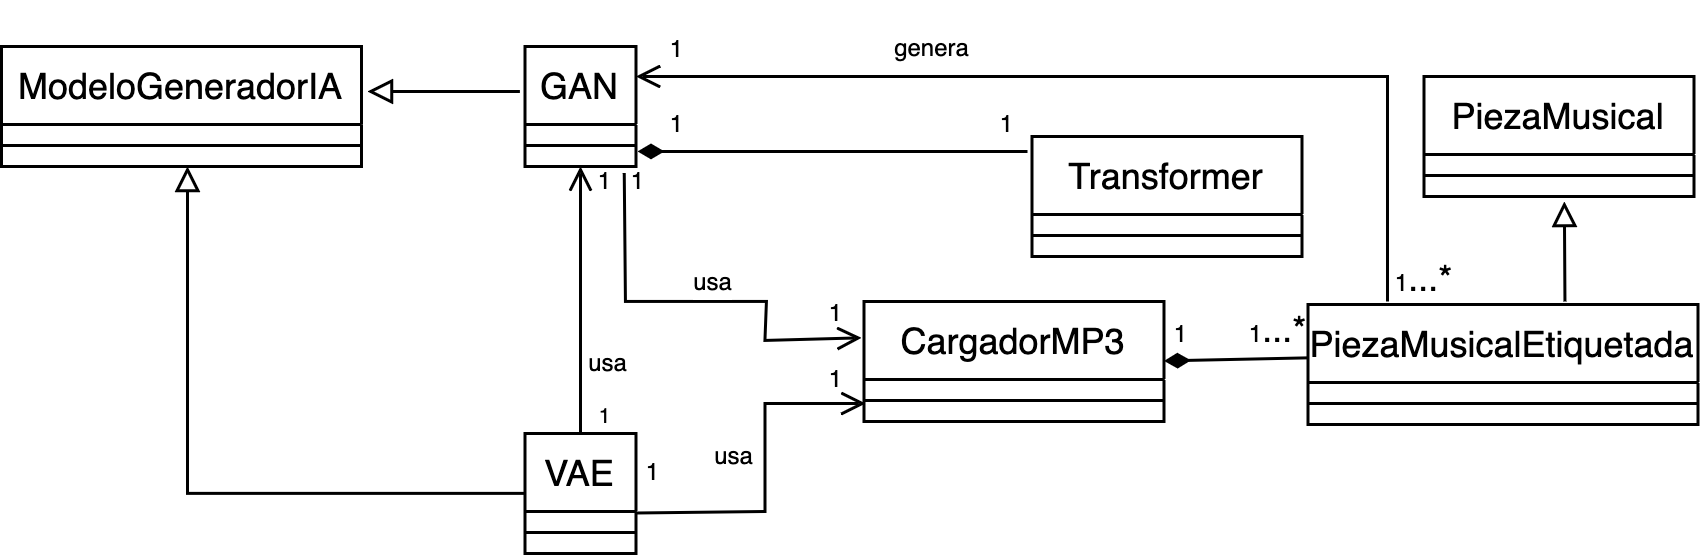
\includegraphics[width=0.9\textwidth]{images/diagrama-clases-ia.png}
    \caption{Diagrama de clases del modelo de Inteligencia Artificial.}
  \end{figure}


  \item \textbf{Diagrama de clases completo}

  \begin{figure}[H]
    \centering
    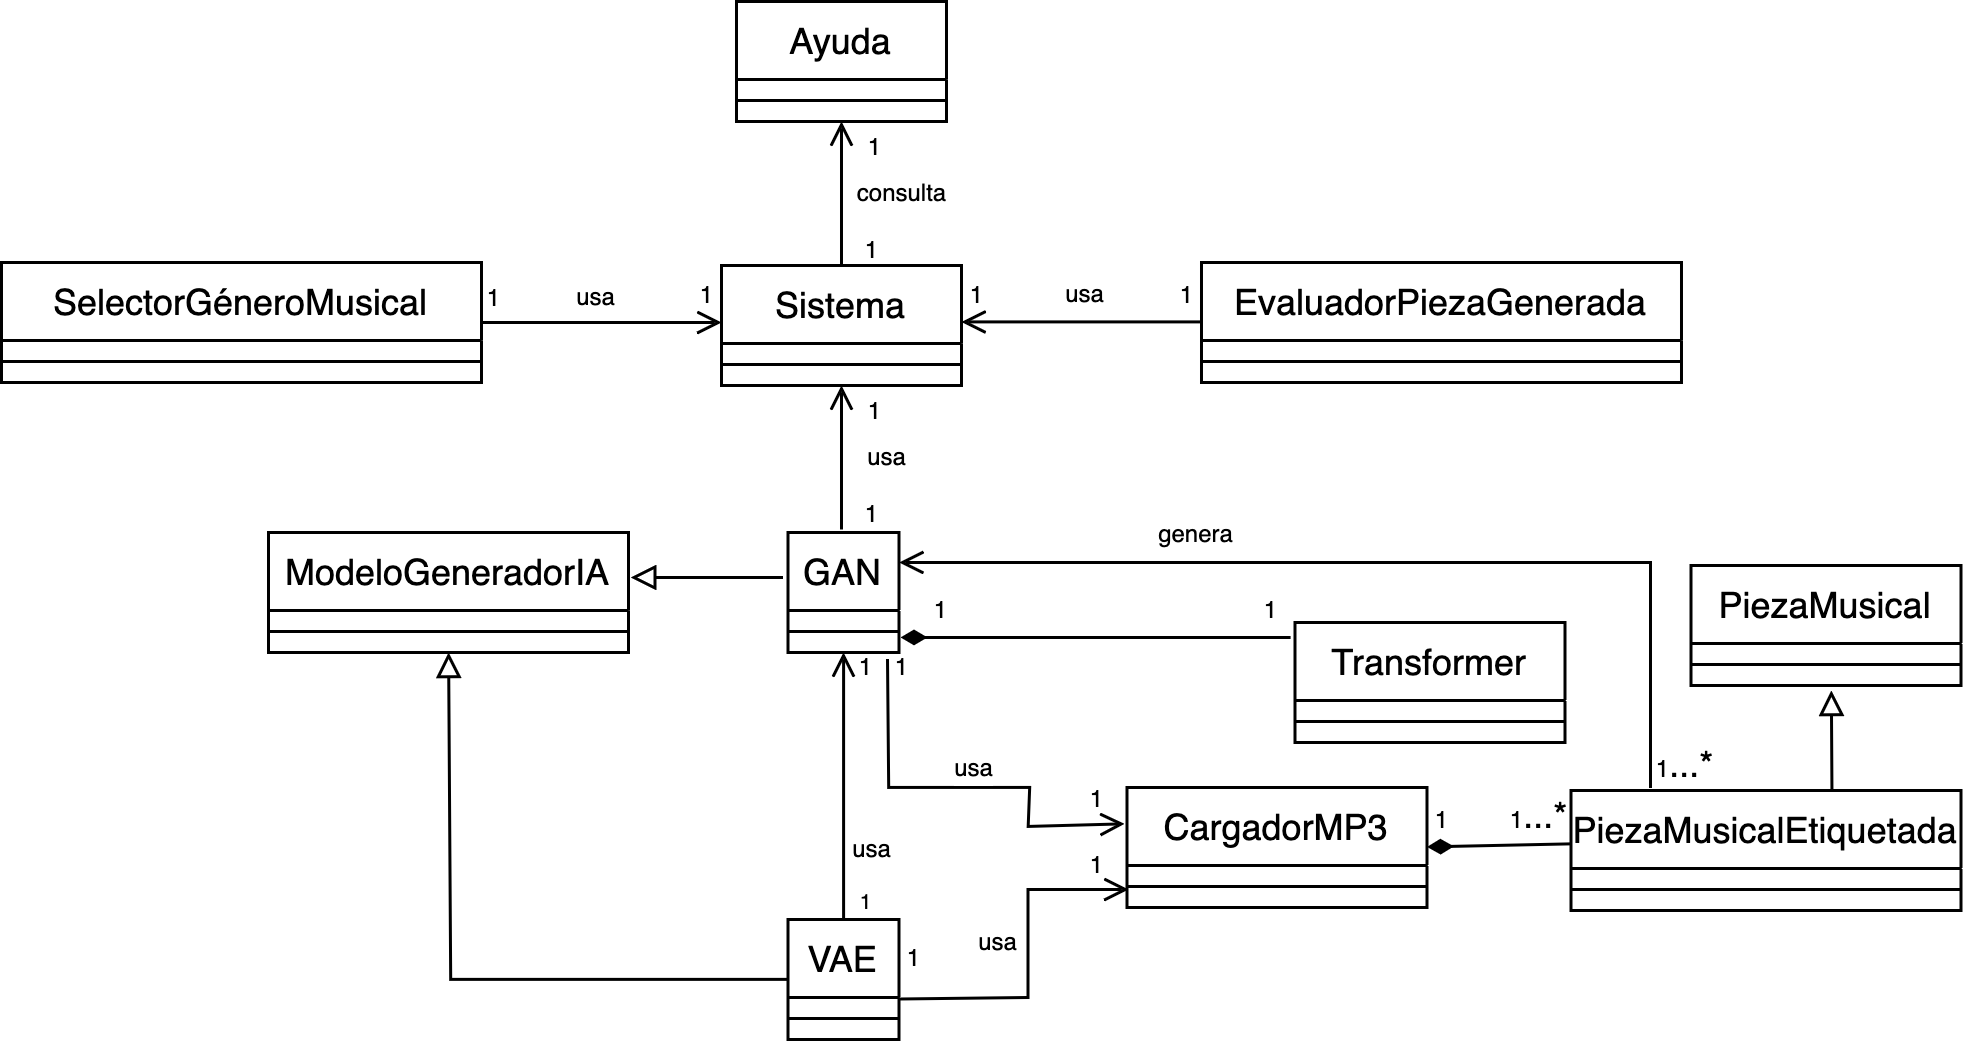
\includegraphics[width=0.9\textwidth]{images/diagrama-clases-completo.png}
    \caption{Diagrama de clases completo.}
  \end{figure}

\end{enumerate}